\documentclass[11pt]{article}

\usepackage[scaled]{helvet}
\renewcommand\familydefault{\sfdefault} 
\usepackage[T1]{fontenc}
\usepackage{url}
\usepackage[breaklinks]{hyperref}
\def\UrlBreaks{\do\/\do-}
\usepackage{siunitx}
\usepackage{hepnames}
\usepackage{hepparticles}
\usepackage{cite}
\usepackage[utf8]{inputenc}
\usepackage[american]{babel}
\usepackage{graphicx}
\usepackage{subcaption}
\usepackage{tikz}
  
% shortcut for location of graphics file
\graphicspath{ {./fig/} }

\usepackage{cite}
\usepackage[top=1in, bottom=1in, left=1in, right=1in, paperwidth=8.5in, paperheight=11in]{geometry}

% some hard-coded definitions for some math symbols to be used more easily
\def \et {E_{T}}
\def \met {\not\!\!\et }
\def \alqed {\alpha_{\mathrm{em}}}
\def \GF {G_{\mathrm{F}}}
\def \mtop {M_{\mathrm{t}}}
\def \mH {M_{\mathrm{H}}}
\def \mX {M_{\mathrm{X}}}
\def \mW {M_{\mathrm{W}}}
\def \mZ {M_{\mathrm{Z}}}
\def \GZ {\Gamma_{\mathrm{Z}}}
\def \GW {\Gamma_{\mathrm{W}}}
\def \WW {{\mathrm{W}^{+}} {\mathrm{W}^{-}} }
\def \ff {\mathrm{f}\mathrm{\overline{f}}}
\def \bb {\mathrm{b}\mathrm{\overline{b}}}
\def \Gt {\Gamma_{\mathrm{t}}}
\def \mt {m_{\mathrm{t}}}
\def \alr {A_{LR}}
\def \alrf {A_{LR}^{f}}
\def \afb {A_{FB}^{f}}
\def \afblr {A_{FB,LR}^{f}}
\def \ee {\mathrm{e}^{+}\mathrm{e}^{-}}
\def \electron {\mathrm{e}^{-}}
\def \positron {\mathrm{e}^{+}}
\def \Jpsi {J/\psi}
\def \KShort {\mathrm{K}^0_{\mathrm{S}}}
\def \Dzero {\mathrm{D}^0}
\def \nZhad {n_{Z^{\mathrm{had}}}}
\def \mumu {\mu^+ \mu^-}
\def \pipi {\pi^+ \pi^-}
\def \pip  {\pi^- \mathrm{p}}
\def \kpi  {\mathrm{K}^- \pi^+}
\def \sweff {{\sin^2{\theta}^{\ell}_{\rm{eff}}}}
\def \sw {\sin^2{\theta}_{\rm{W}}}
\def \ECM {\sqrt{s}}
\def \percmsqs {\mathrm{cm}^{-2}\mathrm{s}^{-1}}
\def \invfb {\mathrm{fb}^{-1}}
\def \invab {\mathrm{ab}^{-1}}
\def \xprime {s^{\prime}/s}
\def \sqrtsp {\sqrt{s}_{p}}
\def \Pel {P_{\mathrm{e^-}}}
\def \Ppos {P_{\mathrm{e^+}}}
\def \SingleWminus {\mathrm{W}^{-} \mathrm{e}^{+} \nu_{\mathrm{e}} }
\def \SingleWplus {\mathrm{W}^{+} \mathrm{e}^{-} \overline{\nu_{\mathrm{e}}} }
\def \g1z {g_{1}^{\mathrm{Z}} }
\def \kgamma {\kappa_{\gamma}}
\def \lgamma {\lambda_{\gamma}}


\title{ \texttt{PHSX815\_Project4}: \\ Employing K-Mean Clustering To The Filtration Of White Light}
\author{~Neno Fuller}
\date{May 2021}

\begin{document}

\maketitle

\section{Introduction \label{sec:intro}}

White-light is a gumbo of many different kinds of 'light' of varying wavelengths. Now, unlike a gumbo where the ingredients are forever entangled to create flavor, white light can be decomposed into its constituents ingredients thorough the use of a filter, the simplest of which is a prism: a transparent material with cut at precise angles and plane faces, and is useful for analyzing and reflecting light ~\cite{Light}. Here in this paper we will simulate a group of filters interacting with white light. This paper is organized as follows: A description of the computer simulation developed to simulate these possibilities is provided in Sec.~\ref{sec:code} with an analysis of the outputs included in Sec.~\ref{sec:analysis}. Finally, conclusions are presented in Sec.~\ref{sec:conclusion}.

\section{Code and Experimental Simulation \label{sec:code}}
The experiment is simulated using a card came. A deck of card is generated and a game is played until one player has all the cards. Each player represents the probability of transmitting light (of any frequencies). Cast in physical terms, imagine you have two or more light filters (“jacks” or "Ace" etc) which allows just a tiny range of wavelengths to pass through. This range is slightly different for each filter. The filters are then placed very close to each other. Then white light (“deck”) is directed to the filters. What you will see on a screen behind the filters are spots with different wavelengths and an overlapping zone between them. In my experiment, I created two classes of filters and ran two simulations. One with just  a single kind of filter (of which there are four) and another with two (for which there are now 8 filters.)

\section{Analysis \label{sec:analysis}}
Figure 1) contains the simulated data. The figure on the left was simulated using 1 kind of filter. Note the dispersing nature of the regions. There is a stronger tendency for shorter frequencies to be filtered. However, because the regions are so concentrated and homogenized, we cannot figure out the locations of the filter and which filtered what wavelength. 

\begin{figure}[htb]
\begin{center}
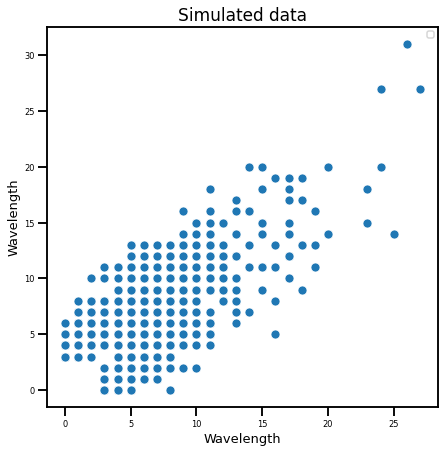
\includegraphics[width=0.49\textwidth]{Figs/Simulated Data.png}
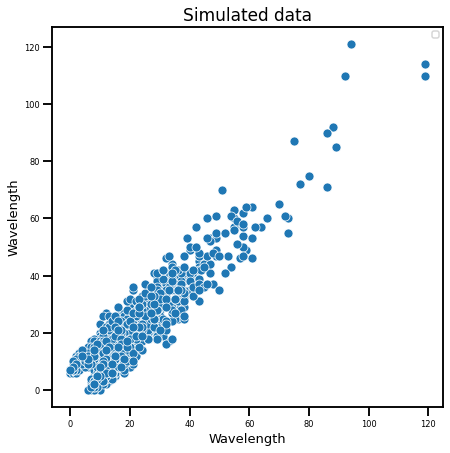
\includegraphics[width=0.49\textwidth]{Figs/SimulatedData2.png}
\caption{{\small Filtered Light: On the left is with 1 Kind of filter, on the right we have two. The modeled locations of the filtered wavelength ranges for each filter are indicated by orange triangles}}
\label{fig:somedata}
\end{center}  
\end{figure}

To surmount this, we apply a K-mean clustering algorithm. Figure 2 contains this information. On the top left we have our simulation of one type of filter using a 2 component mixture model. Now, there are 4 filters of this kind and so, this model fails to capture the data. On the left we see the model with 4 filters. We see the different nature of the filters: we can see the regions of overlap between some of the filters as well as the difference in wavelength regions for each filter. When we create a second class of filters, something interesting happens. The range of each filter and the domain of wavelength filtered condenses. To figure out the respective filters, We first try a 4 component mixture model with the data as show in the bottom left. The bottom right contains an 8 component mixture model which is more accurate given we have 8 filters. As with the simulated data using just one type of filter, we can see features of the general locations of the filters.

\begin{figure*}[htb]
        \centering
        \begin{subfigure}[b]{0.475\textwidth}
            \centering
            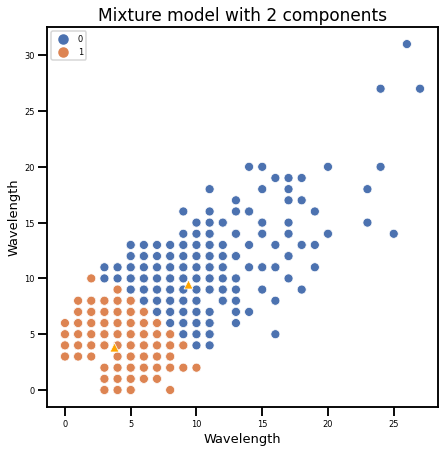
\includegraphics[width=\textwidth]{Figs/Model2Mixture.png}
            \caption[]%
            {{\small }}    
            \label{fig:Biased egeregiously to left}
        \end{subfigure}
        \hfill
        \begin{subfigure}[b]{0.475\textwidth}  
            \centering 
            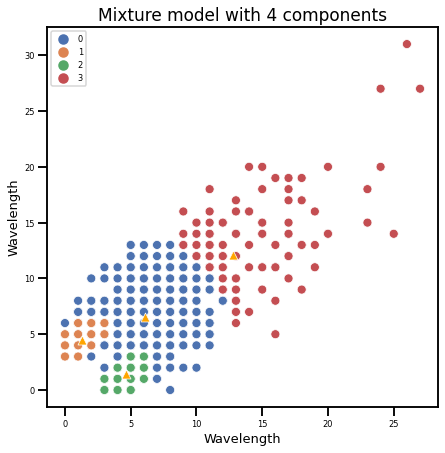
\includegraphics[width=\textwidth]{Figs/Model4Mixture.png}
            \caption[]%
            {{\small }}    
            \label{fig:Biased slightly to left}
        \end{subfigure}
        \vskip\baselineskip
        \begin{subfigure}[b]{0.475\textwidth}   
            \centering 
            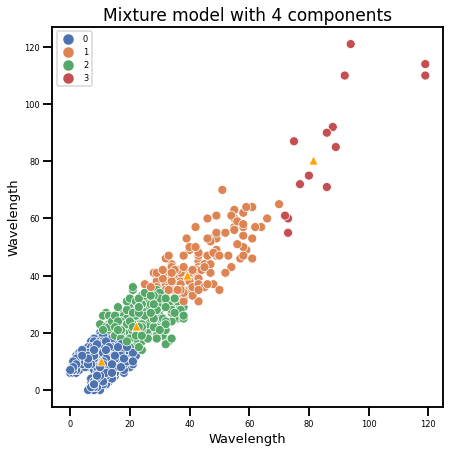
\includegraphics[width=\textwidth]{Figs/Model4Mixture2.png}
            \caption[]%
            {{\small }}    
            \label{fig: Biased slightly to right}
        \end{subfigure}
        \hfill
        \begin{subfigure}[b]{0.475\textwidth}   
            \centering 
            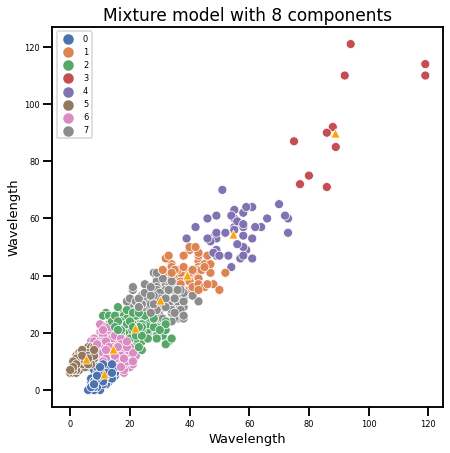
\includegraphics[width=\textwidth]{Figs/Model8Mixture2.png}
            \caption[]%
            {{\small }}    
            \label{fig:Egergiously biased to the right}
        \end{subfigure}
        \caption[Likelihood Estimations]
        {\small Employing K mean clustering to the filtered light }
        \label{fig:LLR}
    \end{figure*}

\section{Conclusion \label{sec:conclusion}}
We employ a rather contrived model to simulate white light being filtered using different filters. We were able to show the wavelength and ranges for which each filter operated. With that, I would like to thank Dr. Rogan and Margaret Lazarovits for making this class incredibly fun and interesting!


\bibliographystyle{unsrt}
\renewcommand{\refname}{References}
\bibliography{main}

\end{document}
